\documentclass[11pt,letterpaper]{article}

%  Paquetes 
\usepackage[utf8]{inputenc}
\usepackage[T1]{fontenc}
\usepackage[spanish,es-tabla,es-nodecimaldot]{babel}
\usepackage{lmodern}
\usepackage[margin=2.5cm]{geometry}
\usepackage{amsmath}
\usepackage{graphicx}
\usepackage{booktabs}
\usepackage{float}
\usepackage{caption}
\usepackage{subcaption}
\usepackage{xcolor}
\usepackage{tikz}
\usetikzlibrary{positioning,arrows.meta}
\usepackage{algorithm}
\usepackage{algpseudocode}
\usepackage[hidelinks]{hyperref}

\floatname{algorithm}{Algoritmo}
\renewcommand{\algorithmicrequire}{\textbf{Entrada:}}
\renewcommand{\algorithmicensure}{\textbf{Salida:}}

%  Portada 
\title{
    \large Instituto Tecnológico de Costa Rica\\
    Escuela de Ingeniería en Computadores\\
    CE 1107: Fundamentos de Arquitectura de Computadores\\[1.2em]
    \Large\textbf{Propuesta de investigación}\\[0.4em]
    \large Costo en área y frecuencia de la descripción estructural frente a la
    descripción de comportamiento en una FPGA Cyclone V
}
\author{
    % Completar con los nombres del grupo
    Jorge Pablo Porras Alvarado \and Marcelo Matey Rodriguez \and Josue Adrian Perez Perez \\[0.8em]
    Profesor: Luis Chavarría Zamora
}
\date{Noviembre de 2026}

\begin{document}

\maketitle

\begin{abstract}
En el Proyecto Grupal 1 todo el sistema de la puerta con contraseña debe describirse de forma
estructural, solo con compuertas y registros, sin \texttt{case}, \texttt{if} ni operadores
aritméticos de alto nivel. Esta investigación mide qué le cuesta esa restricción al circuito que
finalmente se implementa en la FPGA. Se tomaron tres módulos del proyecto (un sumador de
acarreo en cascada, la ALU y el decodificador de siete segmentos), se escribió para cada uno una
versión equivalente de comportamiento (\emph{behavioral}) y se compilaron ambas en Quartus Prime
para una Cyclone~V, con anchos de 4 a 64 bits. Se compararon el área (ALMs y bloques DSP) y la
frecuencia máxima en el modelo de temporización más lento. En el decodificador las dos versiones
resultaron idénticas. En el sumador y la ALU la diferencia es pequeña con pocos bits, pero crece
con el ancho: con 64 bits el sumador estructural es 4.2 veces más lento, y con 32 bits la ALU
estructural ya no cumple el reloj de 50\,MHz del proyecto. Para los anchos que usa el proyecto
(3 a 25 bits) el costo es aceptable.
\end{abstract}

% =====================================================================
\section{Identificación del problema}
% =====================================================================

El enunciado del proyecto exige que el diseño dentro de la FPGA sea estructural: el circuito debe
construirse con ecuaciones booleanas y registros, y no se permiten estructuras de alto nivel como
\texttt{case}, \texttt{if} o el operador ternario~\cite{enunciado}. Por eso, en el proyecto el
sumador se arma con sumadores completos hechos de compuertas, el multiplicador de la ALU es un
arreglo de sumadores y el decodificador del display se escribe como sumas de productos.

Un diseñador que trabaja de forma de comportamiento escribiría lo mismo con \texttt{+},
\texttt{*} o un \texttt{case}, y dejaría que la herramienta de síntesis decida cómo implementarlo.
La pregunta no es trivial por dos razones:

\begin{itemize}
    \item La herramienta de síntesis aplana la jerarquía y minimiza la lógica. Es posible que, al
    final, las dos descripciones terminen en el mismo circuito.
    \item La Cyclone~V tiene recursos dedicados que la herramienta solo usa cuando reconoce una
    operación aritmética: sumadores completos dedicados con una cadena de acarreo rápida dentro de
    cada ALM~\cite{cv_arith}, y bloques DSP para multiplicar~\cite{quartus_mult}. Una descripción
    con compuertas podría no aprovecharlos.
\end{itemize}

El problema, entonces, es saber si diseñar de forma estructural tiene un costo medible en área o
en frecuencia, de qué depende ese costo y si afecta al proyecto. Responderlo permite justificar
con datos el diseño entregado y saber hasta qué tamaño se puede usar este estilo sin problemas.

\subsection*{Objetivo general}
Cuantificar la diferencia en área y frecuencia máxima entre la descripción estructural y la de
comportamiento de módulos combinacionales del proyecto, implementados en una FPGA Cyclone~V.

\subsection*{Objetivos específicos}
\begin{enumerate}
    \item Verificar que cada par de descripciones (estructural y de comportamiento) es funcionalmente
    equivalente.
    \item Medir ALMs, registros, bloques DSP, \emph{slack} de \emph{setup} y frecuencia máxima de
    cada versión para distintos anchos de palabra.
    \item Analizar cómo cambia la diferencia con el ancho y relacionarla con los recursos de la
    arquitectura.
    \item Evaluar si los anchos usados en el proyecto cumplen el reloj de 50\,MHz de la tarjeta.
\end{enumerate}

% =====================================================================
\section{Diseño de la propuesta de investigación}
% =====================================================================

\subsection{Pregunta e hipótesis}

\textbf{Pregunta:} ¿cuánto cambian el área y la frecuencia máxima de un módulo cuando se describe
de forma estructural en lugar de con operadores de comportamiento, y cómo depende ese cambio del
ancho de palabra?

\textbf{Hipótesis:}
\begin{enumerate}
    \item[H1.] En una función combinacional pequeña y sin estructura aritmética, como el
    decodificador de siete segmentos, las dos versiones producen el mismo circuito, porque la
    síntesis reduce ambas a las mismas tablas de búsqueda.
    \item[H2.] En los módulos aritméticos la versión de comportamiento es más rápida, porque la
    herramienta reconoce la suma y la multiplicación y usa la cadena de acarreo y los bloques DSP.
    La diferencia crece con el ancho, ya que el acarreo de un sumador en cascada recorre todos los
    bits~\cite{harris}.
\end{enumerate}

\subsection{Variables}

\begin{table}[H]
\centering
\caption{Variables de la investigación.}
\label{tab:variables}
\begin{tabular}{p{3.2cm}p{11cm}}
\toprule
Tipo & Variables \\
\midrule
Independientes & Estilo de descripción (estructural o de comportamiento); módulo (sumador, ALU,
decodificador); ancho $N$ (4, 8, 16, 32 y 64 bits para el sumador; 4, 8, 16 y 32 para la ALU). \\
Dependientes & ALMs usados; registros; bloques DSP; \emph{slack} de \emph{setup}; frecuencia
máxima $f_{max}$. \\
Controladas & Dispositivo (5CSXFC6D6F31C6); versión de Quartus; reloj de 20\,ns; modelo de
temporización (Slow 1100\,mV 85\,°C); opciones de compilación por defecto; mismo circuito de
prueba alrededor del módulo. \\
\bottomrule
\end{tabular}
\end{table}

\subsection{Módulos bajo prueba}

\begin{table}[H]
\centering
\caption{Pares de módulos comparados.}
\label{tab:modulos}
\begin{tabular}{p{2.6cm}p{6cm}p{6cm}}
\toprule
Módulo & Versión estructural (del proyecto) & Versión de comportamiento \\
\midrule
Sumador & Cadena de $N$ sumadores completos, cada uno con compuertas XOR, AND y OR. &
Suma con el operador de suma sobre $N+1$ bits. \\
ALU & Suma y resta con el mismo sumador en cascada, multiplicación por arreglo de sumadores,
rotaciones con multiplexores por etapas, selección del resultado con multiplexores. &
Las mismas cinco operaciones con operadores de suma, resta, multiplicación y desplazamiento, y
selección con una estructura de casos. \\
Decodificador & Suma de productos por segmento (los dígitos donde el segmento se apaga). &
Tabla de 16 casos. \\
\bottomrule
\end{tabular}
\end{table}

Las versiones de comportamiento se escribieron solo para esta investigación y no forman parte del
diseño entregado.

\subsection{Metodología}

\paragraph{Paso 1: equivalencia funcional.} Antes de medir, se comprueba en simulación que cada
par produce las mismas salidas para todas las entradas posibles. Sin este paso, una diferencia en
área o velocidad podría deberse a que los módulos no hacen lo mismo.

\paragraph{Paso 2: circuito de prueba.} Cada módulo se coloca entre dos bancos de registros
(Figura~\ref{fig:banco}). Así el analizador de temporización mide el camino de registro a
registro, que es justamente el retardo del módulo. Las entradas y salidas se declaran como pines
virtuales para no depender de la ubicación de los pines físicos, lo que además permite probar
anchos grandes que no cabrían en los pines de la tarjeta. Los registros son los mismos en las dos
versiones, así que no afectan la comparación.

\begin{figure}[H]
\centering
\begin{tikzpicture}[every node/.style={align=center},
    caja/.style={draw, thick, minimum height=1.4cm, minimum width=2.2cm, align=center},
    flecha/.style={-{Stealth[length=2.5mm]}, thick},
    node distance=1.2cm]
    \node (in)  {Pines\\virtuales};
    \node[caja, right=of in]  (r1)  {Registros\\de entrada};
    \node[caja, right=of r1, fill=gray!15, minimum width=2.8cm] (dut) {Módulo bajo\\prueba};
    \node[caja, right=of dut] (r2)  {Registros\\de salida};
    \node[right=of r2] (out) {Pines\\virtuales};
    \draw[flecha] (in) -- (r1);
    \draw[flecha] (r1) -- (dut);
    \draw[flecha] (dut) -- (r2);
    \draw[flecha] (r2) -- (out);
    \node[below=0.5cm of dut] (clk) {Reloj de 50\,MHz (20\,ns)};
    \draw[flecha, dashed] (clk.west) -| (r1.south);
    \draw[flecha, dashed] (clk.east) -| (r2.south);
    \draw[thick, draw=gray, {Bar[]}-{Bar[]}] ([yshift=0.35cm]r1.north east) -- node[above]{camino medido} ([yshift=0.35cm]r2.north west);
\end{tikzpicture}
\caption{Circuito de prueba usado para cada módulo.}
\label{fig:banco}
\end{figure}

\paragraph{Paso 3: compilación automatizada.} Un \emph{script} en Tcl ejecutado con
\texttt{quartus\_sh} crea el proyecto, asigna el dispositivo, los archivos, la restricción de reloj
y los pines virtuales, fija los parámetros $N$ y la variante, y ejecuta síntesis, ajuste
(\emph{fitter}) y análisis de temporización. Luego lee los reportes y guarda una fila por
compilación en un archivo CSV. El Algoritmo~\ref{alg:flujo} resume el procedimiento.

\begin{algorithm}[H]
\caption{Flujo de compilación y medición}
\label{alg:flujo}
\begin{algorithmic}[1]
\Require lista de módulos, anchos de cada módulo, variantes \{estructural, comportamiento\}
\Ensure archivo de resultados con área y temporización
\For{cada módulo $m$}
    \For{cada ancho $N$ de $m$}
        \For{cada variante $v$}
            \State crear un proyecto nuevo para la Cyclone V con el circuito de prueba de $m$
            \State asignar reloj de 20\,ns, pines virtuales y los parámetros $N$ y $v$
            \State ejecutar síntesis, \emph{fitter} y análisis de temporización
            \State leer ALMs, registros y DSP del resumen del \emph{fitter}
            \State leer el \emph{slack} de \emph{setup} del modelo Slow 1100\,mV 85\,°C
            \State calcular $f_{max} = 1/(T - \text{slack})$ y escribir la fila en el archivo
        \EndFor
    \EndFor
\EndFor
\end{algorithmic}
\end{algorithm}

\paragraph{Paso 4: métricas.} El área se toma como el número de ALMs (Adaptive Logic Modules), la
unidad lógica básica de la Cyclone~V~\cite{alm}, junto con los bloques DSP. La velocidad se toma
del \emph{slack} de \emph{setup}, del que se obtienen el retardo del camino crítico y la
frecuencia máxima:
\begin{equation}
    t_{camino} = T - \text{slack}, \qquad f_{max} = \frac{1}{T - \text{slack}}, \qquad T = 20\,\text{ns}.
    \label{eq:fmax}
\end{equation}
Se usa el modelo Slow 1100\,mV 85\,°C porque es el peor caso de temperatura y voltaje del
dispositivo.

\subsection{Herramientas}
\begin{itemize}
    \item Quartus Prime Lite Edition 25.1std.0, dispositivo Cyclone~V SX 5CSXFC6D6F31C6 (el de la
    tarjeta DE10-Standard).
    \item Analizador de temporización de Quartus (\emph{Timing Analyzer}).
    \item \emph{Script} en Tcl ejecutado con \texttt{quartus\_sh} para automatizar las 20
    compilaciones.
    \item Simulador Verilator para la prueba de equivalencia.
    \item Python con Matplotlib para las gráficas.
\end{itemize}

% =====================================================================
\section{Ejecución de la metodología}
% =====================================================================

\subsection{Equivalencia funcional}

La prueba de equivalencia recorrió todas las combinaciones de entrada de cada par
(Tabla~\ref{tab:equiv}).

\begin{table}[H]
\centering
\caption{Casos revisados en la prueba de equivalencia.}
\label{tab:equiv}
\begin{tabular}{lrr}
\toprule
Par comparado & Casos & Diferencias \\
\midrule
Sumador de 4 bits (todas las $a$, $b$ y acarreo de entrada) & 512 & 0 \\
Sumador de 8 bits & 131\,072 & 0 \\
ALU de 3 bits (todas las $a$, $b$ y los 8 códigos de operación) & 512 & 0 \\
ALU de 4 bits & 2\,048 & 0 \\
Decodificador (los 16 valores) & 16 & 0 \\
\bottomrule
\end{tabular}
\end{table}

En la primera ejecución aparecieron diferencias en la ALU, solo con el código de operación
\texttt{110}, que el proyecto no usa. La ALU estructural decodifica la operación bit a bit, de
modo que ese código termina seleccionando la rotación a la derecha, mientras que la primera
versión de comportamiento devolvía cero. Se ajustó la versión de comportamiento para que
reprodujera ese caso y, con ese cambio, todas las combinaciones coincidieron. Este resultado
confirma la importancia del paso 1: sin él se habrían comparado dos circuitos distintos.

\subsection{Compilación}

Se ejecutaron 20 compilaciones: 10 del sumador, 8 de la ALU y 2 del decodificador. La
Tabla~\ref{tab:resultados} reúne los datos obtenidos.

\begin{table}[H]
\centering
\caption{Resultados de compilación (modelo Slow 1100\,mV 85\,°C, reloj de 20\,ns). El retardo
y la $f_{max}$ se calculan con la ecuación~\eqref{eq:fmax}.}
\label{tab:resultados}
\small
\setlength{\tabcolsep}{4pt}
\begin{tabular}{llrrrrrrr}
\toprule
Módulo & $N$ & Variante & ALMs & Registros & DSP & Slack (ns) & Retardo (ns) & $f_{max}$ (MHz) \\
\midrule
Sumador & 4 & Estructural & 11 & 14 & 0 & 18.172 & 1.828 & 547.05 \\
Sumador & 4 & Behavioral & 10 & 14 & 0 & 18.104 & 1.896 & 527.43 \\
Sumador & 8 & Estructural & 22 & 26 & 0 & 16.438 & 3.562 & 280.74 \\
Sumador & 8 & Behavioral & 18 & 26 & 0 & 17.658 & 2.342 & 426.99 \\
Sumador & 16 & Estructural & 44 & 50 & 0 & 15.143 & 4.857 & 205.89 \\
Sumador & 16 & Behavioral & 34 & 50 & 0 & 16.880 & 3.120 & 320.51 \\
Sumador & 32 & Estructural & 91 & 98 & 0 & 10.082 & 9.918 & 100.83 \\
Sumador & 32 & Behavioral & 66 & 98 & 0 & 16.277 & 3.723 & 268.60 \\
Sumador & 64 & Estructural & 181 & 194 & 0 & 5.000 & 15.000 & 66.67 \\
Sumador & 64 & Behavioral & 130 & 194 & 0 & 16.446 & 3.554 & 281.37 \\
\midrule
ALU & 4 & Estructural & 31 & 19 & 0 & 15.679 & 4.321 & 231.43 \\
ALU & 4 & Behavioral & 32 & 19 & 1 & 14.061 & 5.939 & 168.38 \\
ALU & 8 & Estructural & 108 & 31 & 0 & 11.922 & 8.078 & 123.79 \\
ALU & 8 & Behavioral & 79 & 31 & 1 & 13.815 & 6.185 & 161.68 \\
ALU & 16 & Estructural & 328 & 55 & 0 & 3.519 & 16.481 & 60.68 \\
ALU & 16 & Behavioral & 176 & 55 & 1 & 10.660 & 9.340 & 107.07 \\
ALU & 32 & Estructural & 1132 & 103 & 0 & -8.179 & 28.179 & 35.49 \\
ALU & 32 & Behavioral & 378 & 103 & 2 & 9.397 & 10.603 & 94.31 \\
\midrule
Decodificador & 4 (fijo) & Estructural & 10 & 11 & 0 & 18.785 & 1.215 & 823.05 \\
Decodificador & 4 (fijo) & Behavioral & 10 & 11 & 0 & 18.785 & 1.215 & 823.05 \\
\bottomrule
\end{tabular}
\end{table}

Para validar el cálculo de la ecuación~\eqref{eq:fmax}, se comparó con el reporte \emph{Fmax
Summary} de Quartus en la última compilación (decodificador): la ecuación da 823.05\,MHz, igual
que la columna \emph{Fmax} del reporte. Ese mismo reporte indica una \emph{Restricted Fmax} de
717.36\,MHz, limitada por el periodo mínimo del reloj. La \emph{Restricted Fmax} toma en cuenta
restricciones que la \emph{Fmax} no considera, como el ancho mínimo de pulso, y nunca es mayor
que ella~\cite{sta_fmax}. Por eso, los valores de la tabla por encima de unos 717\,MHz sirven
para comparar las dos versiones, pero no son frecuencias que el dispositivo pueda alcanzar.

% =====================================================================
\section{Análisis de los datos}
% =====================================================================

\subsection{Decodificador de siete segmentos}

Las dos versiones usaron 10 ALMs y dieron exactamente el mismo \emph{slack} (18.785\,ns). Esto
confirma la hipótesis H1: para una función de cuatro entradas y siete salidas, la síntesis reduce
la suma de productos y la tabla de casos a las mismas tablas de búsqueda, y el estilo de
descripción no influye en el resultado.

\subsection{Sumador}

\begin{figure}[H]
\centering
\begin{subfigure}{0.49\textwidth}
    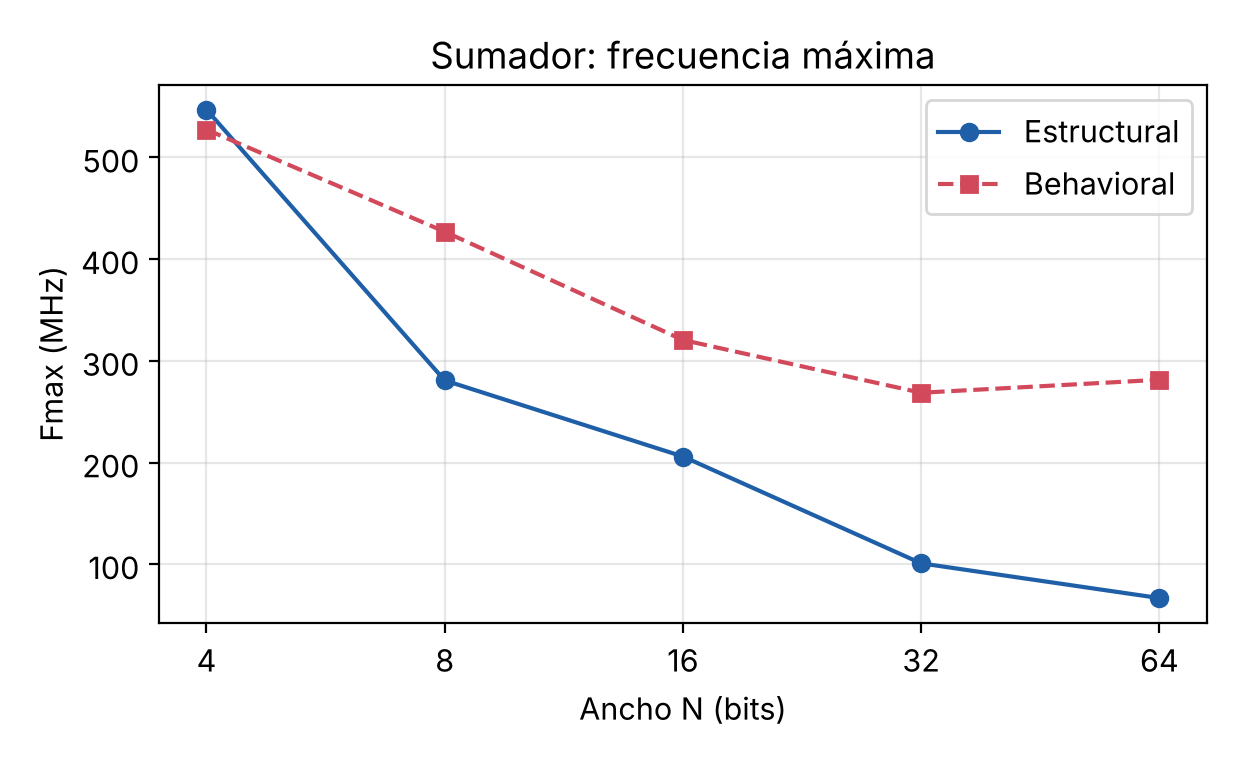
\includegraphics[width=\linewidth]{figuras/fmax_sumador.png}
    \caption{Frecuencia máxima.}
\end{subfigure}
\hfill
\begin{subfigure}{0.49\textwidth}
    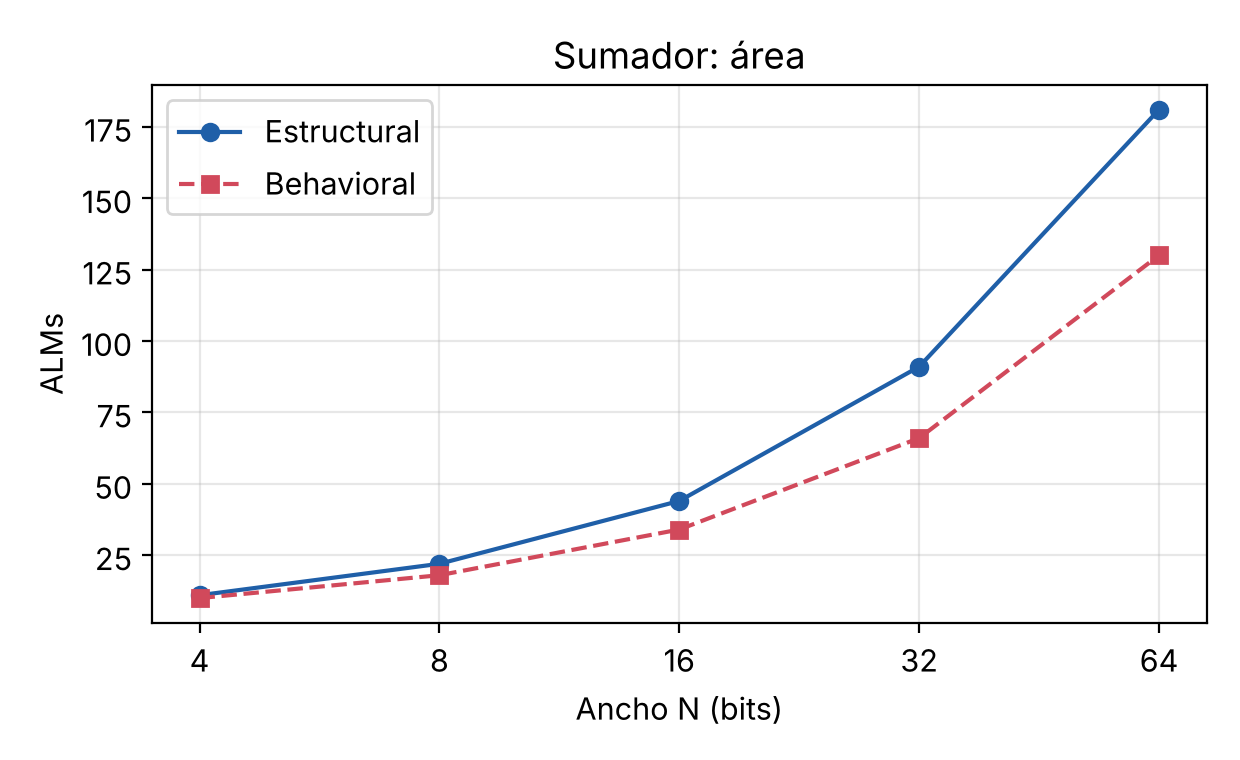
\includegraphics[width=\linewidth]{figuras/area_sumador.png}
    \caption{Área.}
\end{subfigure}
\caption{Sumador estructural y de comportamiento contra el ancho $N$.}
\label{fig:sumador}
\end{figure}

Con 4 bits las dos versiones son prácticamente iguales (547 y 527\,MHz). A partir de ahí se
separan (Figura~\ref{fig:sumador}):

\begin{itemize}
    \item El retardo de la versión estructural crece casi en proporción al ancho: pasa de
    1.83\,ns con $N=4$ a 15.00\,ns con $N=64$, unos 0.22\,ns por bit. Es el comportamiento
    esperado de un sumador en cascada, en el que el acarreo atraviesa todos los bits~\cite{harris}.
    \item El retardo de la versión de comportamiento casi no cambia: se mantiene entre 1.9 y
    3.7\,ns, y su $f_{max}$ queda alrededor de 270 a 280\,MHz desde $N=32$.
    \item La razón entre las frecuencias crece con el ancho: 1.5 veces con $N=8$, 2.7 veces con
    $N=32$ y 4.2 veces con $N=64$.
    \item En área, la versión estructural usa entre 2.75 y 2.84 ALMs por bit, contra unos 2 de la
    de comportamiento; con $N=64$ son 181 contra 130 ALMs (1.4 veces más).
\end{itemize}

La explicación más probable está en la arquitectura. Cada ALM de la Cyclone~V tiene, en modo
aritmético, dos sumadores completos dedicados y una cadena de acarreo rápida que conecta ALMs
vecinos~\cite{cv_arith}. Cuando la herramienta reconoce una suma, como en la versión de
comportamiento, usa esa cadena, y el acarreo avanza por un camino dedicado muy corto. En la
versión estructural el acarreo se describe con compuertas, de modo que se implementa con tablas
de búsqueda comunes y viaja por el ruteo general. Esto explica a la vez la pendiente del retardo
y el área extra.

\subsection{ALU}

\begin{figure}[H]
\centering
\begin{subfigure}{0.49\textwidth}
    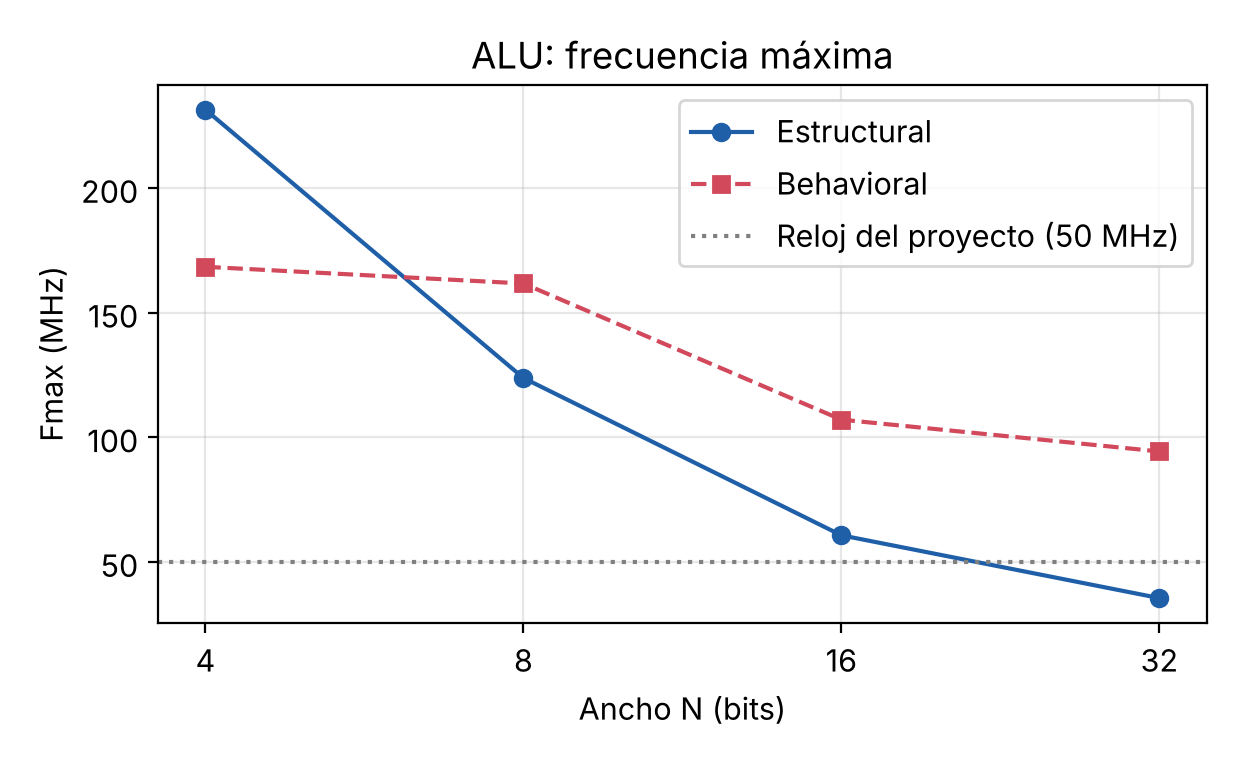
\includegraphics[width=\linewidth]{figuras/fmax_alu.png}
    \caption{Frecuencia máxima.}
\end{subfigure}
\hfill
\begin{subfigure}{0.49\textwidth}
    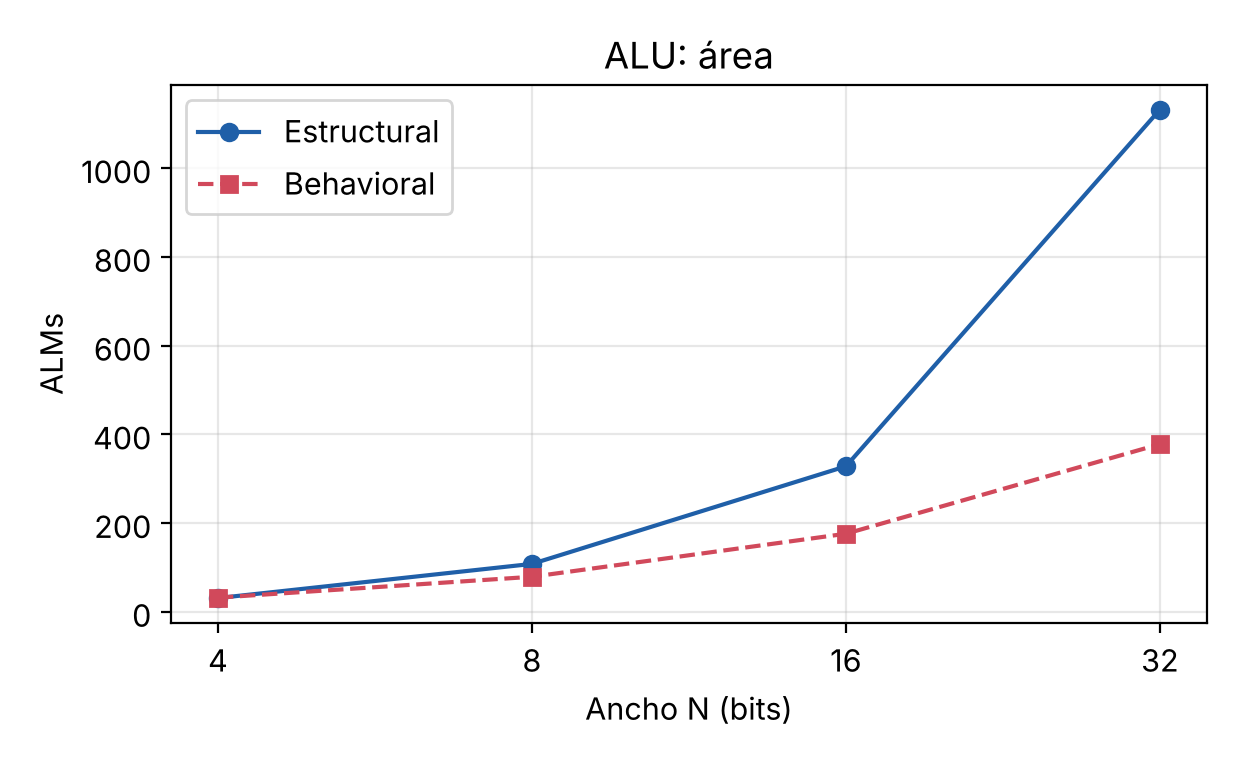
\includegraphics[width=\linewidth]{figuras/area_alu.png}
    \caption{Área.}
\end{subfigure}
\caption{ALU estructural y de comportamiento contra el ancho $N$.}
\label{fig:alu}
\end{figure}

La ALU muestra el caso más marcado (Figura~\ref{fig:alu}):

\begin{itemize}
    \item \textbf{Con $N=4$ gana la versión estructural} (231\,MHz contra 168\,MHz). La versión
    de comportamiento implementa la multiplicación en un bloque DSP~\cite{quartus_mult}, y el
    trayecto de entrada y salida del bloque agrega retardo. Para un multiplicador tan pequeño, la
    lógica en tablas de búsqueda es más rápida.
    \item \textbf{Desde $N=8$ gana la versión de comportamiento}, y la ventaja crece: 1.3 veces
    con $N=8$, 1.8 veces con $N=16$ y 2.7 veces con $N=32$.
    \item \textbf{El área estructural crece mucho más rápido.} Pasa de 31 a 1\,132 ALMs cuando el
    ancho pasa de 4 a 32 bits, unas 36 veces más con un ancho 8 veces mayor, lo que se acerca a un
    crecimiento cuadrático. Se debe al multiplicador por arreglo: son $N$ sumadores de $2N$ bits.
    La versión de comportamiento pasa de 32 a 378 ALMs, porque la multiplicación ocupa 1 o 2
    bloques DSP en vez de lógica.
    \item \textbf{Con $N=32$ la ALU estructural no cumple el reloj del proyecto.} Su
    \emph{slack} es de $-8.179$\,ns: el camino crítico tarda 28.18\,ns, más que el periodo de
    20\,ns, y su $f_{max}$ es de 35.5\,MHz. La versión de comportamiento sí cumple, con 94.3\,MHz.
\end{itemize}

La Figura~\ref{fig:retardo} reúne el retardo de los cuatro casos: solo la ALU estructural cruza
el periodo de 20\,ns.

\begin{figure}[H]
\centering
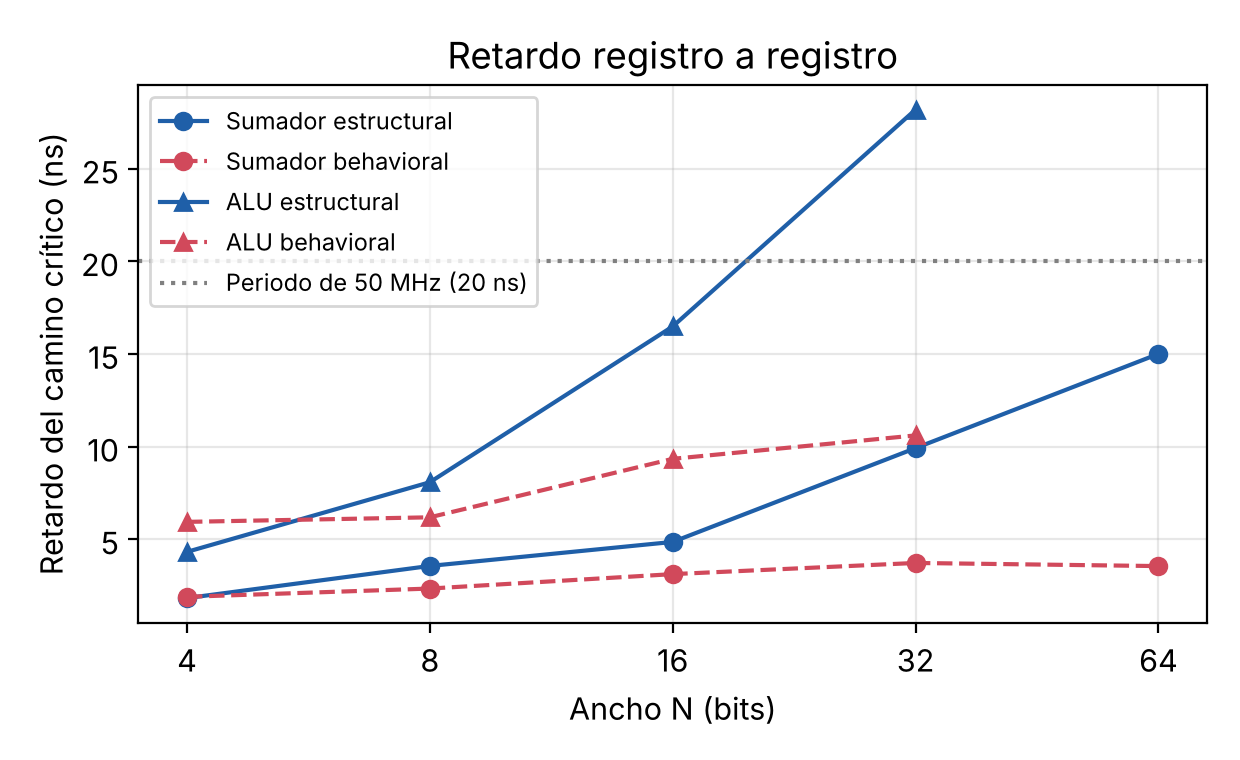
\includegraphics[width=0.75\textwidth]{figuras/retardo.png}
\caption{Retardo del camino crítico de cada versión contra el ancho, comparado con el periodo
del reloj del proyecto.}
\label{fig:retardo}
\end{figure}

\subsection{Relación con el proyecto}

Los módulos del proyecto trabajan con anchos pequeños: la ALU y el PWM usan 3 bits, el divisor
de reloj del PWM 15 bits y el temporizador de sonidos 25 bits. En ese rango los datos muestran
que la descripción estructural no tiene un costo importante:

\begin{itemize}
    \item La ALU de 4 bits estructural fue incluso más rápida que la de comportamiento, y con la
    misma área.
    \item El sumador estructural de 16 bits alcanza 206\,MHz y el de 32 bits 101\,MHz, así que un
    contador de 25 bits queda entre esos valores, muy por encima de los 50\,MHz de la tarjeta.
\end{itemize}

\subsection{Limitaciones}

\begin{itemize}
    \item Se usó un solo dispositivo y una sola versión de Quartus. Otras familias, con otros
    recursos dedicados, pueden dar resultados distintos.
    \item Se hizo una sola compilación por caso, con las opciones por defecto. El \emph{fitter}
    tiene una componente aleatoria (la semilla de ubicación), así que cada valor puede variar unos
    pocos por ciento entre ejecuciones.
    \item El número de ALMs incluye los registros del circuito de prueba. Son los mismos en las dos
    versiones, así que no cambian la comparación, pero sí el valor absoluto.
    \item Las versiones de comportamiento son directas, sin optimizaciones especiales. Un diseño
    más cuidado podría ser aún más rápido.
\end{itemize}

% =====================================================================
\section{Conclusiones}
% =====================================================================

\begin{enumerate}
    \item La descripción estructural no siempre tiene un costo. En una función combinacional
    pequeña, como el decodificador de siete segmentos, la síntesis produjo exactamente el mismo
    circuito con las dos descripciones.
    \item En los circuitos aritméticos el costo existe y crece con el ancho. Con 64 bits, el
    sumador estructural fue 4.2 veces más lento y usó 1.4 veces más área. Con 32 bits, la ALU
    estructural fue 2.7 veces más lenta, usó 3 veces más ALMs y no cumplió el reloj de 50\,MHz.
    \item La causa principal es que la herramienta solo usa la cadena de acarreo dedicada y los
    bloques DSP cuando reconoce la operación aritmética. Escrita con compuertas, la misma
    operación se implementa con lógica general y ruteo.
    \item Los recursos dedicados no siempre ganan: con 4 bits, la ALU estructural fue más rápida,
    porque el retardo de entrar y salir del bloque DSP pesa más que la multiplicación misma.
    \item Para los anchos del proyecto (3 a 25 bits), la restricción de diseñar de forma
    estructural no compromete el funcionamiento: todos los módulos cumplen con holgura el reloj
    de 50\,MHz. Si en un proyecto futuro se necesitaran palabras de 32 bits o más, convendría
    estructurar los sumadores para aprovechar la cadena de acarreo, o reconsiderar el estilo de
    descripción.
\end{enumerate}

% =====================================================================
\begin{thebibliography}{9}

\bibitem{enunciado}
L.~Chavarría Zamora, \emph{Proyecto Grupal 1: Máquinas de estados}, CE 1107 Fundamentos de
Arquitectura de Computadores, Instituto Tecnológico de Costa Rica, 2026.

\bibitem{cv_arith}
Intel Corporation, ``Arithmetic Mode,'' en \emph{Cyclone V Device Handbook, Volume 1: Device
Interfaces and Integration}. [En línea]. Disponible:
\url{https://www.intel.com/content/www/us/en/docs/programmable/683375/current/arithmetic-mode.html}

\bibitem{alm}
Intel Corporation, ``ALM Resources,'' en \emph{Cyclone V Device Handbook, Volume 1: Device
Interfaces and Integration}. [En línea]. Disponible:
\url{https://www.intel.com/content/www/us/en/docs/programmable/683375/current/alm-resources.html}

\bibitem{quartus_mult}
Intel Corporation, ``Inferring Multipliers,'' en \emph{Intel Quartus Prime Standard Edition User
Guide: Design Recommendations}, v18.1. [En línea]. Disponible:
\url{https://www.intel.com/content/www/us/en/docs/programmable/683323/18-1/inferring-multipliers.html}

\bibitem{sta_fmax}
Intel Corporation, ``Report Fmax Summary,'' en \emph{Intel Quartus Prime Pro Edition User Guide:
Timing Analyzer}, v23.3. [En línea]. Disponible:
\url{https://www.intel.com/content/www/us/en/docs/programmable/683243/23-3/report-fmax-summary.html}

\bibitem{harris}
D.~M. Harris y S.~L. Harris, \emph{Digital Design and Computer Architecture}, 2.ª ed.
Waltham, MA, EE.~UU.: Morgan Kaufmann, 2012.

\end{thebibliography}

\end{document}
